Έγινε εκτέλεση των δύο υλοποιήσεων στα web graphs των \textcite{snapnets}.
Εδώ παρουσιάζονται διαγράμματα με διάφορα χαρακτηριστικά των εκτελέσεων για
web graph με 875.713 κόμβους με 4.563.235 συνδέσμους στα ακόλουθα συστήματα:
\begin{enumerate}

\item 4 πύρηνο σύστημα
\begin{itemize}
\item Intel(R) Core(TM) i5-4670 CPU @ 3.40GHz.
\item 8GB DDR3 RAM
\item gcc version 7.3.0
\end{itemize}

\item 8 πύρηνο σύστημα (diades)
\begin{itemize}
\item Intel(R) Xeon(R) CPU E5420  @ 2.50GHz.
\item 8GB DDR3 RAM
\item gcc version 5.4.0
\end{itemize}
\end{enumerate}


\begin{center}
\begin{figure}
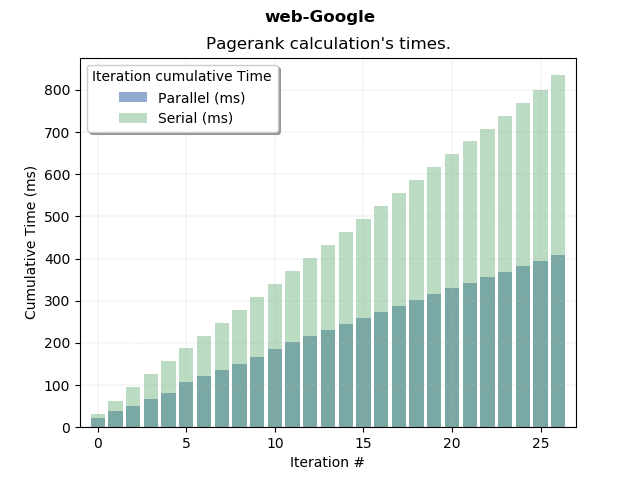
\includegraphics[width=\linewidth]{plots/it_time.png}
\caption{Χρονική εξέλιξη των δύο υλοποιήσεων. 4-πύρηνο σύστημα.}
\end{figure}

\begin{figure}
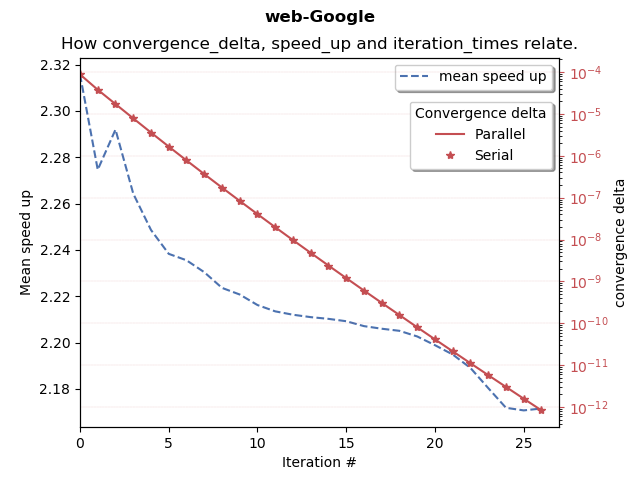
\includegraphics[width=\linewidth]{plots/speed_up.png}
\caption{Σχέση σταθεράς σύγκλισης, επιτάχυνσης και αριθμού επαναλήψεων. 4-πύρηνο σύστημα.}
\label{fig:relat}
\end{figure}

\begin{figure}
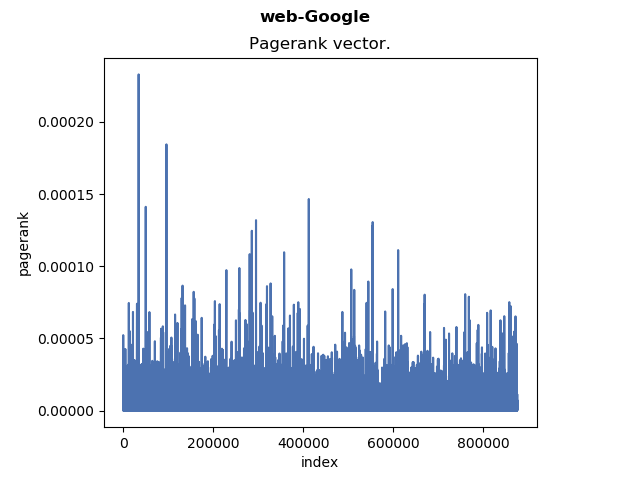
\includegraphics[width=\linewidth]{plots/pagerank.png}
\caption{Το αποτέλεσμα για κάθε κόμβο.}
\end{figure}

\begin{figure}
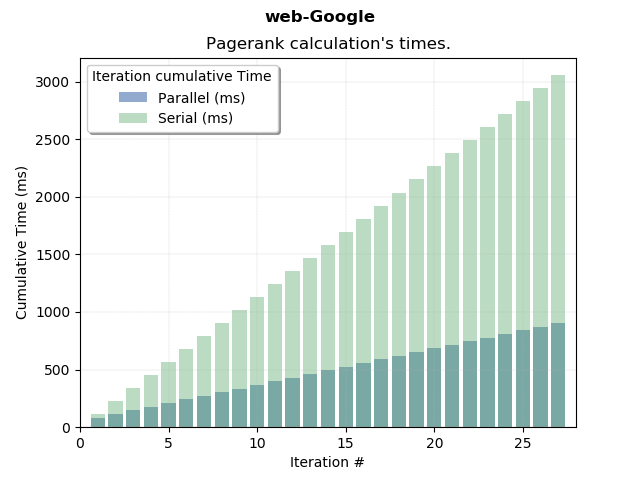
\includegraphics[width=\linewidth]{plots/it_times_diades.png}
\caption{Χρονική εξέλιξη των δύο υλοποιήσεων. 8-πύρηνο σύστημα.}
\end{figure}

\begin{figure}
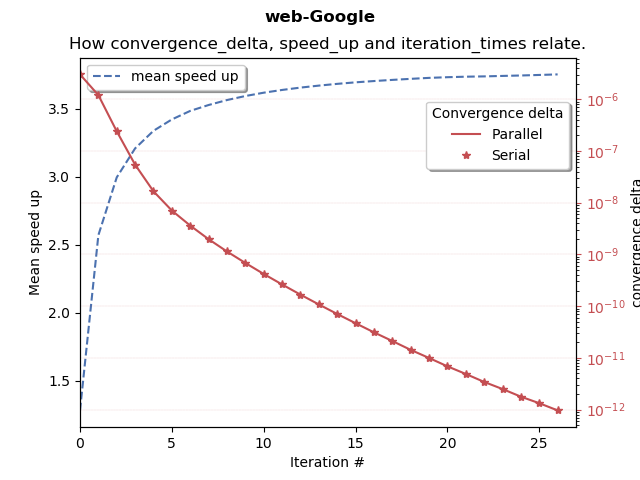
\includegraphics[width=\linewidth]{plots/speed_up_diades.png}
\caption{Σχέση σταθεράς σύγκλισης, επιτάχυνσης και αριθμού επαναλήψεων. 8-πύρηνο σύστημα.}
\label{fig:relatd}
\end{figure}

\begin{figure}
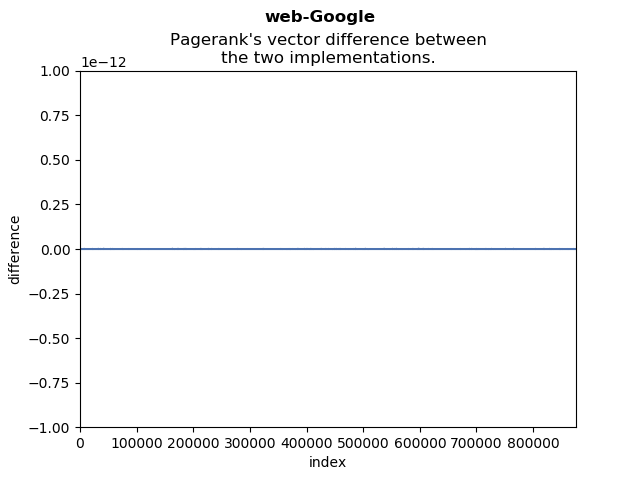
\includegraphics[width=\linewidth]{plots/diff.png}
\caption{Διαφορά των δύο υλοποιήσεων στο τελικό διάνυσμα.}
\label{fig:dif}
\end{figure}

\end{center}


Αποτελέσματα και για τα υπόλοιπα web-graphs συμπεριλαμβάνονται στα παραδοτέα. Γενικώς, παρατηρήθηκε ικανοποιητική επιτάχυνση με ταχύτητα τουλάχιστον 2 φορές μεγαλύτερη για την παράλληλη υλοποίηση στο τετραπύρηνο σύστημα ή/και έως 3,5 φορές μεγαλύτερη στο οκταπύρηνο σύστημα. Αντίστοιχα καλές επιδόσεις παρατηρήθηκαν για όλα τα σετ δεδομένων με εξαίρεση το web-BerkStan graph όπου ο edge-coloring αλγόριθμος δημιούργησε ιδιαίτερα αυξημένο αριθμό ομάδων.

Σε όλες τις περιπτώσεις, η παράλληλη υλοποίηση του αλγορίθμου «στοχαστικοποίησης» των στηλών του γράφου για την δημιουργία του πίνακα $\bm{A}_s$ ήταν σαφώς ταχύτερη από τη σειριακή.
